\documentclass[11pt]{article}

\usepackage[margin=1in]{geometry}
\usepackage{microtype}
\usepackage{amsmath}
\usepackage{graphicx}
\usepackage{booktabs}
\usepackage[hidelinks]{hyperref}

\graphicspath{{figures/}}

\newcommand{\natex}{\texttt{natex}}

\title{Manufactured Gradients: State AI Exposure and US Business AI
Adoption at DeepSeek-R1}
\author{Hauke Hillebrandt\thanks{University College London. Email:
\texttt{ucjthhi@ucl.ac.uk}. This paper and the underlying \natex{} software were
prepared with substantial assistance from Anthropic's Claude models; the author
reviewed the analyses and text and is responsible for all remaining errors.}}
\date{July 2026 \\ \small analysis pass of record: 2026-07, \natex{} v0.2.0, seed 0}

\begin{document}

\maketitle

\begin{abstract}
\noindent US states more exposed to AI --- measured by the Anthropic Economic
Index (AEI) usage-per-capita index --- did not detectably accelerate business
AI adoption relative to less-exposed states at the release of DeepSeek-R1 on
20 January 2025. In Census Bureau Business Trends and Outlook Survey (BTOS)
state panels (2{,}727 state-wave cells, 51 states, 71 biweekly waves,
2023--2026), the change in each state's adoption-trend slope at R1 rises by
$+1.635$ pp/yr per AEI index unit (HC1 se $1.458$) --- reproducing the scout
estimate to the third decimal --- but is statistically null:
exposure-permutation $p=0.257$. The same statistic at non-event placebo
cutoffs brackets the headline ($+1.56$ at $t=2024.30$, $+2.24$ at $2024.50$),
and a placebo \emph{outcome} --- remote work, whose federal return-to-office
executive order was signed the same day as R1 --- matches it ($+1.97$), with
the weighted placebo version itself nominally significant ($p=0.045$): the
design manufactures gradients. Every nominally significant estimate in the
battery traces to a known mechanism. Long-window negative gradients ($-4.31$
at $w=1.0$) vanish under old-wording-only data --- a splice artifact, because
the nationally calibrated $1.553$ rewording ratio misprices high-adoption,
high-AEI states (corr $+0.676$). The two-way fixed-effects level effect
($+0.527$ pp, permutation $p=0.011$) is a pre-trend: the high-minus-low gap
was already growing at $+0.600$ pp/yr before R1, and state-specific trends
flip the estimate to $-0.38$. The scan's localization at the first post-R1
wave is a mechanical rediscovery of the constructed treatment column. There
is no credible evidence that high-AEI-exposure states accelerated AI adoption
differentially at DeepSeek-R1: the BTOS state Bartik-style design, excluded
from an earlier screen for want of exposure weights, stays dead even with
real ones.
\end{abstract}

\section{Introduction}\label{sec:intro}

The release of the DeepSeek-R1 reasoning model on 20 January 2025
\cite{guo2025} is the natural candidate event for a break in US business AI
adoption: a companion sector-level analysis \cite{hillebrandt2026r1} of the
Census Bureau's Business Trends and Outlook Survey (BTOS) found a sharp
acceleration in AI-exposed sectors at exactly the first post-R1 survey wave,
but attribution to R1 failed a placebo battery. This paper asks the
cross-sectional version of the same question: did \emph{states} whose
workforces use AI more intensively accelerate measured business AI adoption
differentially at R1? The design --- state-level BTOS adoption interacted
with an external AI-exposure measure --- was excluded from an earlier
automated screen for want of exposure weights; here we revive it with real
ones.

Both sides of the design rest on new measurement. The outcome is the BTOS AI
use rate, a biweekly probability-sample estimate of the share of US firms
using AI, introduced and validated by \cite{bonney2024}. The exposure is the
Anthropic Economic Index (AEI), which maps Claude conversations to economic
tasks \cite{handa2025}; its geographic report \cite{appel2025} publishes a
usage-per-capita index by US state, which we take as the cross-state
exposure measure. Interacting differential exposure with a common shock is
the logic that shift-share (Bartik) designs formalize
\cite{goldsmithpinkham2020}, and its known failure modes discipline the
analysis: exposure here is measured \emph{after} the outcome window, so every
estimate below is a descriptive gradient, never a causal Bartik coefficient;
pre-existing differential trends can masquerade as treatment effects
\cite{roth2022}; and slope changes at a single date in smooth aggregate
series are spuriously significant often enough that placebo distributions at
non-event dates, in the spirit of \cite{ganong2018}, are the appropriate
yardstick. The per-state slope-change contrast is a kink-style estimand in
the sense of the difference-in-kinks design \cite{bockerman2025}, estimated
and falsified with the \natex{} toolkit \cite{natex}, whose scan-based DiD
\cite{herlands2018} supplies a localization check. The battery converts one
reproduced headline gradient and three nominally significant side results
into a clean null plus three identified artifacts.

\section{Data}\label{sec:data}

The outcome panel combines three BTOS sources. The state sheets of the AI
core workbook (DRB approval CBDRB-FY25-0425) give biweekly estimates and
standard errors of the share answering ``Yes'' to Question~7 (``In the last
two weeks, did this business use Artificial Intelligence (AI) in producing
goods or services?''), waves 202319--202520. A fresh census.gov download
extends the panel under the December-2025 rewording (``\ldots in any of its
business activities?''), waves 202524--202614; new-wording values are divided
by $1.553$, the national new/old measurement-RDD ratio estimated at the
rewording cutoff by a companion paper \cite{hillebrandt2026rewording}, with
an additive $-6.04$ pp variant as a diagnostic. The archived remote-work
Question~6 (share of businesses with paid employees working from home at
least one workday), waves 202417--202514, supplies a placebo outcome (1{,}221
state-wave cells). The assembled panel has 2{,}727 state-wave cells across 51
states (50 plus DC) and 71 waves, $t=2023.710$--$2026.507$ in fractional
years of collection-period midpoints; $24.7\%$ of the state-by-wave grid is
disclosure-suppressed, concentrated in small states.

Exposure is the AEI \texttt{usage\_per\_capita\_index} per state
\cite{appel2025}, averaged over the 2026-04-01..05-01 and 2026-05-01..06-01
data windows (verified: CA $=(1.56+1.62)/2=1.59$); it ranges from $3.52$ (DC)
to $0.245$ (WV). Two features bind the interpretation. First, the exposure
window (April--June 2026) lies entirely \emph{after} the outcome window, so
exposure is endogenous by construction and no estimate below is causal,
whatever its $p$-value. Second, the index measures Claude usage specifically,
proxying all-AI exposure with attenuation and tech-hub confounding both
plausible.

\section{Design and Methods}\label{sec:methods}

\paragraph{Exposure gradient at a known cutoff.} For each state $s$, local
OLS slopes of the adoption share in calendar time are fit on each side of
$t_0=2025.055$ (DeepSeek-R1; first post wave 202503) within $\pm w$ years,
and the slope change $\Delta\kappa_s$ is the post-minus-pre difference ---
the right-minus-left kink convention of \cite{bockerman2025}, with the
cross-state gradient replacing the group contrast. The headline statistic is
the cross-state regression of $\Delta\kappa_s$ on AEI exposure, $b$ in pp/yr
per index unit. The spec of record is $w=0.5$, unweighted, restricted to
states with at least 6 usable waves per side ($n=36$; DC never enters ---
it is suppressed below the wave minimum). Inference is primary by exposure
permutation (AEI values reassigned across states, $B=10{,}000$,
\texttt{default\_rng(0)}), with HC1 standard errors reported alongside
\cite{cameron2015}; windows $w\in\{0.5, 0.75, 1.0, 1.4\}$ are examined, and
an SE-weighted variant fits $1/\mathrm{se}^2$ WLS slopes from the published
State SE sheets and combines them by inverse-variance meta-analysis.

\paragraph{Falsification battery.} (i) placebo cutoffs at the non-event dates
$2024.30$ and $2024.50$, at o1 ($2024.6967$, a real secondary event), at
$2025.30$, and at $2025.555$ (a window that straddles the rewording splice);
(ii) the placebo outcome (remote work) at the R1 cutoff --- noting that the
federal return-to-office executive order was signed on 2025-01-20, the
\emph{same day} as R1, so remote-work breaks at that date are expected for
non-AI reasons; (iii) leverage checks dropping DC and CA, and a Spearman rank
gradient; (iv) splice diagnostics rerunning the long-window gradients under
the multiplicative ($/1.553$) splice, the additive ($-6.04$ pp) splice, and
old-wording-only data ($t<2025.8$).

\paragraph{Panel estimators.} A tercile two-way fixed-effects (TWFE) level
DiD interacts the top AEI tercile (17 states, cut $1.002$) with post-R1,
with wave and state fixed effects, CR1 standard errors by state
\cite{cameron2015}, a placebo-in-space permutation of the treated set
($B=2{,}000$), and a state-specific linear-trends variant. The \natex{}
survey pipeline's scan-based DiD (SuDDDS) \cite{herlands2018} searches break
dates and windows on the same panel (seed 0, normal model, AR(1)-by-unit
permutation null) as a localization and role-assignment check.

\paragraph{Honest-inference notes, stated as run.} HC1/CR1 intervals on
smooth biweekly aggregates are potentially oversized, so permutation $p$ is
the primary inference throughout. The \natex{} refusals are reported, not
patched over: the SuDDDS anticipation test refused (Holm $p$ all NaN), and
all three effect estimators (dd, synthetic control, GESS) refused with
``only 0 usable placebos; $\geq 5$ required'' on this unbalanced panel ---
the manual TWFE and permutation estimates below are the effect numbers of
record.

\section{Results}\label{sec:results}

\begin{figure}[t]
\centering
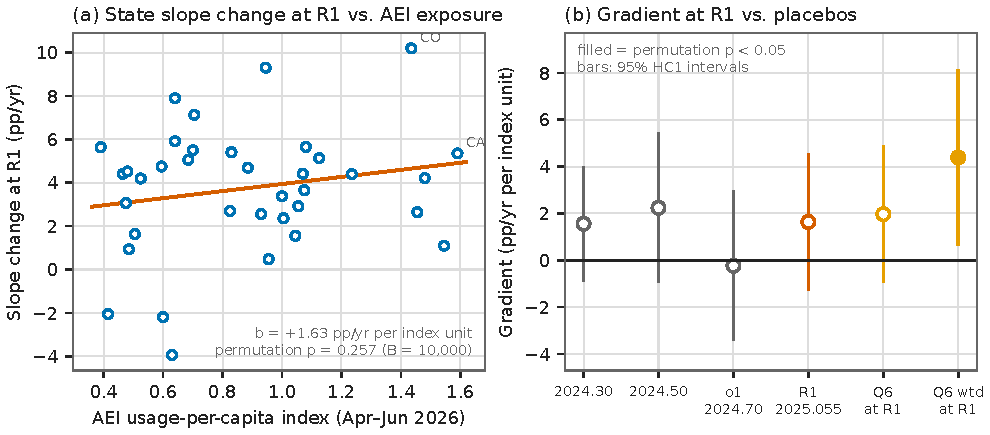
\includegraphics[width=\textwidth]{fig1}
\caption{(a) State-level slope change in BTOS AI use at DeepSeek-R1
($w=\pm 0.5$ yr, $n=36$ states with $\geq 6$ waves per side) against AEI
usage-per-capita exposure, with the unweighted OLS fit: $b=+1.635$ pp/yr per
index unit, exposure-permutation $p=0.257$. (b) The same gradient statistic
at non-event placebo cutoffs, at o1, at R1, and for the remote-work placebo
outcome at R1, with 95\% HC1 intervals; filled markers are nominally
significant by permutation at the 5\% level. The only filled marker in the
battery is a \emph{placebo} --- the SE-weighted remote-work gradient at R1
($+4.39$, $p=0.045$).}
\label{fig:fig1}
\end{figure}

\paragraph{The scout number reproduces exactly, and it is null.} At the spec
of record ($w=0.5$, unweighted, 36 states), the R1 slope-change gradient is
$b=+1.635$ pp/yr per AEI index unit (HC1 se $1.458$; classical se $1.428$,
matching the scout's ``se 1.43, $t$ 1.15''; $t_{\mathrm{HC1}}=1.12$;
correlation $0.193$), with exposure-permutation $p=0.257$
(Table~\ref{tab:main}, panel A; Figure~\ref{fig:fig1}a). The SE-weighted
version is $+1.877$ (HC1 se $1.922$, $p_{\mathrm{perm}}=0.360$); the
Spearman rank gradient is $\rho=0.098$ ($p=0.568$); dropping DC and CA gives
$+1.54$ ($p=0.326$) unweighted and $+0.53$ ($p=0.804$) weighted. DC --- the
highest-exposure unit at AEI $3.52$ --- never enters the gradient sample in
the first place, so no single unit drives the (non-)result.

\paragraph{Placebos bracket the headline.} The identical statistic at
non-event cutoffs returns $+1.56$ ($p=0.277$) at $t=2024.30$ and $+2.24$
($p=0.162$) at $t=2024.50$ --- magnitudes that \emph{bracket} the R1
estimate --- and $-0.23$ ($p=0.889$) at o1 (Table~\ref{tab:main}, panel B;
Figure~\ref{fig:fig1}b). The remote-work placebo outcome at R1 is $+1.97$
($p=0.288$), the same magnitude as the headline; its SE-weighted version is
$+4.39$ (HC1 se $1.895$) with permutation $p=0.045$ --- a nominally
significant \emph{placebo}. A design that produces R1-sized gradients at
dates where nothing happened, and a significant gradient for an outcome
whose own policy shock (the federal return-to-office executive order, signed
2025-01-20) merely shares R1's date, manufactures gradients; the null at R1
carries no information beyond that.

\paragraph{Artifact 1: the long-window sign flip is the splice.} Once the
window reaches across the December-2025 rewording, the gradient turns
significantly negative: $-4.31$ ($p=0.011$) at $w=1.0$ and $-2.53$
($p=0.011$) at $w=1.4$ (Table~\ref{tab:main}, panel C). This is a
measurement artifact, identified three ways. AEI exposure correlates
$+0.676$ with the pre-R1 adoption level, so the nationally calibrated
multiplicative ratio $1.553$ misprices high-level (equivalently high-AEI)
states; the additive $-6.04$ pp splice --- wrong in the opposite direction
--- attenuates the same estimates to $-2.92$ and $-1.07$; and
old-wording-only data collapse both to null ($-0.87$, $p=0.279$ at $w=1.0$;
$+0.44$, $p=0.513$ at $w=1.4$). A placebo cutoff at $2025.555$, placed so
the window straddles the splice with no event nearby, yields $-9.16$
($p=0.00025$) multiplicative and still $-5.81$ ($p=0.015$) additive:
\emph{neither} national correction is valid cross-state, so state-level
gradients through the rewording --- including any June-2026 extension of
this design --- are unidentified.

\paragraph{Artifact 2: the TWFE level effect is a pre-trend.} The tercile
TWFE DiD gives $\hat\tau=+0.527$ pp (CR1 se $0.210$) with placebo-in-space
permutation $p=0.011$ ($+0.547$, $p=0.038$ on the full panel) --- nominally
the strongest result in the study (Table~\ref{tab:main}, panel D). But the
high-minus-low AEI gap was already growing at $+0.600$ pp/yr before R1 (HC1
se $0.180$, 36 pre-R1 waves), which mechanically predicts roughly $+0.3$ pp
of the estimate over the post window, and adding state-specific linear
trends flips the $w=0.5$ estimate to $-0.38$ (se $0.31$). This is the
textbook pre-trend failure \cite{roth2022}: the level DiD is descriptive
only, and the trend-robust estimand --- the slope-change gradient --- is
exactly the null of panel A.

\paragraph{Artifact 3: the scan localization is treatment rediscovery.} The
SuDDDS scan (seed 0, both panels) maximizes at LLR $154.5$ for the empty
subset --- \emph{all} states --- at $t_0=2025.0877$, the first post-R1 wave,
with scan $p=0.010$ under the AR(1)-by-unit null. Because the declared
treatment column is the constructed \texttt{high\_aei}$\times$\texttt{post}
indicator, a scan that lights up for all states at the post boundary is a
mechanical rediscovery of that column, not outcome evidence --- the same
role-assignment failure documented in the companion sector study
\cite{hillebrandt2026r1}. The composition check passes ($p=0.707$); the
anticipation test and all three effect estimators refused, as stated in
Section~\ref{sec:methods}.

\begin{table}[t]
\centering
\scriptsize
\caption{Exposure gradients, placebos, and panel estimates. Gradient rows:
slope-change gradient $b$ (pp/yr per AEI index unit) with HC1 se and
exposure-permutation $p$ ($B=10{,}000$; splice diagnostics $B=4{,}000$).
TWFE rows: level effect (pp) with CR1 se by state and placebo-in-space
permutation $p$ ($B=2{,}000$).}
\label{tab:main}
\begin{tabular}{lrrrr}
\toprule
Specification & Estimate & se & $p_{\mathrm{perm}}$ & $n$ \\
\midrule
\multicolumn{5}{l}{\emph{Panel A: AEI gradient at DeepSeek-R1 ($w=0.5$ yr)}}\\
unweighted (spec of record)        & $+1.635$ & $1.458$ & $0.257$ & 36 \\
SE-weighted (WLS $+$ IV meta)      & $+1.877$ & $1.922$ & $0.360$ & 36 \\
unweighted, drop DC$+$CA           & $+1.544$ & $1.651$ & $0.326$ & 35 \\
SE-weighted, drop DC$+$CA          & $+0.531$ & $2.316$ & $0.804$ & 35 \\
\midrule
\multicolumn{5}{l}{\emph{Panel B: placebo cutoffs and placebo outcome ($w=0.5$, unweighted)}}\\
placebo cutoff $t_0=2024.30$       & $+1.560$ & $1.224$ & $0.277$ & 33 \\
placebo cutoff $t_0=2024.50$       & $+2.238$ & $1.604$ & $0.162$ & 34 \\
o1 cutoff $t_0=2024.6967$          & $-0.233$ & $1.610$ & $0.889$ & 33 \\
remote work (Q6) at R1             & $+1.970$ & $1.458$ & $0.288$ & 51 \\
remote work (Q6) at R1, SE-weighted & $+4.392$ & $1.895$ & $0.045^{\ast}$ & 51 \\
\midrule
\multicolumn{5}{l}{\emph{Panel C: long windows across the 2025-12 rewording (unweighted)}}\\
$w=1.0$, spliced ($/1.553$)        & $-4.305$ & $1.676$ & $0.011^{\ast}$ & 39 \\
$w=1.0$, additive splice ($-6.04$ pp) & $-2.922$ & $1.885$ & $0.020^{\ast}$ & 39 \\
$w=1.0$, old wording only          & $-0.873$ & $1.000$ & $0.279$ & 39 \\
$w=1.4$, spliced                   & $-2.535$ & $0.945$ & $0.011^{\ast}$ & 40 \\
$w=1.4$, old wording only          & $+0.439$ & $0.645$ & $0.513$ & 40 \\
splice-window placebo $t_0=2025.555$, spliced & $-9.161$ & $2.150$ & $0.00025^{\ast}$ & 39 \\
splice-window placebo, additive    & $-5.806$ & $2.639$ & $0.015^{\ast}$ & 39 \\
\midrule
\multicolumn{5}{l}{\emph{Panel D: tercile TWFE level DiD (pp)}}\\
TWFE, $w=0.5$                      & $+0.527$ & $0.210$ & $0.011^{\ast}$ & 964 \\
TWFE, full panel                   & $+0.547$ & $0.236$ & $0.038^{\ast}$ & 2727 \\
TWFE $+$ state trends, $w=0.5$     & $-0.382$ & $0.315$ & --- & 964 \\
pre-R1 high-minus-low gap slope (pp/yr) & $+0.600$ & $0.180$ & --- & 36 waves \\
\bottomrule
\end{tabular}

\medskip
\parbox{0.92\textwidth}{\footnotesize Notes: $^{\ast}$ nominally significant
at the 5\% level by permutation. The $w=1.4$ additive-splice gradient is
$-1.069$ ($p=0.095$). Panel D's TWFE $p$-values are placebo-in-space; the
state-trends row and the pre-trend slope row report CR1 and HC1 standard
errors respectively, with no permutation test run. Every nominally
significant row is attributed to an identified artifact in the text: splice
mispricing (panel C), a pre-existing differential trend (panel D), or a
same-day policy shock to the placebo outcome (panel B).}
\end{table}

\section{Caveats and Conclusion}\label{sec:conclusion}

Four caveats bound the claims. First, \emph{exposure is post-outcome}: the
AEI index is measured April--June 2026, after every outcome wave used at the
R1 cutoff, so even a robust gradient would have been descriptive, not
Bartik-causal --- the null is about this gradient design, not proof of zero
differential adoption. Second, \emph{exposure is Claude-specific}: as a
proxy for all-AI exposure it is attenuated and plausibly confounded with
tech-hub geography. Third, \emph{coverage}: $24.7\%$ of the state-wave grid
is disclosure-suppressed, concentrated in small states; estimation samples
run 33--40 states, and DC --- the most exposed unit --- is never estimable
at the primary window. Fourth, \emph{the calendar}: R1's release week was
inauguration week, sharing its date with the federal return-to-office
executive order (2025-01-20) and adjoining the Stargate announcement
(2025-01-21), the AI-diffusion export rule (2025-01-13), and a BTOS
sample-year rollover, so even a surviving gradient could not have been
attributed to R1 alone.

The conclusion is a disciplined null. The headline gradient reproduces
exactly and is statistically indistinguishable from the same statistic at
dates where nothing happened; the one nominally significant gradient in the
$w=0.5$ battery belongs to a placebo outcome with its own same-day shock;
and all three seemingly significant side results --- the long-window
negative gradients, the TWFE level effect, and the scan localization ---
dissolve under, respectively, old-wording-only data, state trends, and
role-assignment scrutiny. These data provide no credible evidence that
high-AEI-exposure states accelerated business AI adoption differentially at
DeepSeek-R1, and the state-level splice problem implies that extending the
design through the rewording cannot rescue it.

\paragraph{Reproducibility.} All estimates were produced with \natex{}
v0.2.0 \cite{natex} at seed 0 from the frozen BTOS workbooks (published at
\url{https://www.census.gov/hfp/btos}) and the public AEI state release
\cite{appel2025}; no dataset files are committed. Figure~\ref{fig:fig1}
regenerates deterministically from the committed
\texttt{figures/make\_fig.py}, which asserts the headline gradient and the
significant-placebo numbers against the numbers of record before drawing.

\footnotesize
\begin{thebibliography}{9}
\setlength{\itemsep}{1pt}\setlength{\parskip}{0pt}

\bibitem{appel2025}
Appel, R., McCrory, P., Tamkin, A., McCain, M., Neylon, T., and Stern, M.
(2025).
Anthropic Economic Index report: Uneven geographic and enterprise AI
adoption.
arXiv:2511.15080.

\bibitem{bockerman2025}
B\"ockerman, P., Jysm\"a, S., and Kanninen, O. (2025).
\emph{Difference-in-Kinks Design}.
IZA Discussion Paper No.~18313.
\url{https://docs.iza.org/dp18313.pdf}

\bibitem{bonney2024}
Bonney, K., Breaux, C., Buffington, C., Dinlersoz, E., Foster, L.,
Goldschlag, N., Haltiwanger, J., Kroff, Z., and Savage, K. (2024).
Tracking firm use of AI in real time: A snapshot from the Business Trends
and Outlook Survey.
NBER Working Paper No.~32319.

\bibitem{cameron2015}
Cameron, A.~C., and Miller, D.~L. (2015).
A practitioner's guide to cluster-robust inference.
\emph{Journal of Human Resources}, 50(2), 317--372.

\bibitem{ganong2018}
Ganong, P., and J\"ager, S. (2018).
A permutation test for the regression kink design.
\emph{Journal of the American Statistical Association}, 113(522), 494--504.

\bibitem{goldsmithpinkham2020}
Goldsmith-Pinkham, P., Sorkin, I., and Swift, H. (2020).
Bartik instruments: What, when, why, and how.
\emph{American Economic Review}, 110(8), 2586--2624.

\bibitem{guo2025}
Guo, D., Yang, D., Zhang, H., et al. (2025).
DeepSeek-R1 incentivizes reasoning in LLMs through reinforcement learning.
\emph{Nature}, 645(8081), 633--638.

\bibitem{handa2025}
Handa, K., Tamkin, A., McCain, M., et al. (2025).
Which economic tasks are performed with AI? Evidence from millions of Claude
conversations.
arXiv:2503.04761.

\bibitem{herlands2018}
Herlands, W., McFowland~III, E., Wilson, A.~G., and Neill, D.~B. (2018).
Automated local regression discontinuity design discovery.
In \emph{Proceedings of the 24th ACM SIGKDD International Conference on
Knowledge Discovery and Data Mining (KDD~'18)}.

\bibitem{hillebrandt2026r1}
Hillebrandt, H. (2026).
A sharp bend, no verdict: Difference-in-kinks tests of US business AI
adoption at DeepSeek-R1.
Companion paper, natex paper collection.
\url{https://haukehillebrandt.github.io/natex/btos-sector-did-r1/}

\bibitem{hillebrandt2026rewording}
Hillebrandt, H. (2026).
The question is the treatment: A known-cutoff regression discontinuity at
the BTOS AI-question rewording.
Companion paper, natex paper collection.
\url{https://haukehillebrandt.github.io/natex/btos-rewording-rdd/}

\bibitem{natex}
Hillebrandt, H. (2026).
\emph{natex: automated natural-experiment discovery and estimation} (version
0.2.0). Software.
\url{https://github.com/HaukeHillebrandt/natex}

\bibitem{roth2022}
Roth, J. (2022).
Pretest with caution: Event-study estimates after testing for parallel
trends.
\emph{American Economic Review: Insights}, 4(3), 305--322.

\end{thebibliography}

\end{document}
